\documentclass[xcolor=x11names,compress]{beamer}

%% General document %%%%%%%%%%%%%%%%%%%%%%%%%%%%%%%%%%
\usepackage{graphicx}
\usepackage{svg}
\usepackage{tikz}
\usetikzlibrary{decorations.fractals}
\usetikzlibrary{arrows.meta}
\usetikzlibrary{3d}
\usetikzlibrary{positioning}
\usetikzlibrary{fit}
\usetikzlibrary{shapes}
\usetikzlibrary{shapes.geometric}
\usetikzlibrary{shapes.misc}
\usetikzlibrary{backgrounds}
\usetikzlibrary{arrows.meta}
%%%%%%%%%%%%%%%%%%%%%%%%%%%%%%%%%%%%%%%%%%%%%%%%%%%%%%


%% Beamer Layout %%%%%%%%%%%%%%%%%%%%%%%%%%%%%%%%%%
\useoutertheme[subsection=false,shadow]{miniframes}
\useinnertheme{default}
\usefonttheme{serif}
\usepackage{palatino}
\usepackage{setspace,textcomp,soul}
\usepackage{beamerprosper}

\setbeamerfont{title like}{shape=\scshape}
\setbeamerfont{frametitle}{shape=\scshape}
\definecolor{bluUnicam}{RGB}{27,43,74}
\definecolor{redUnicam}{RGB}{219,0,36}
\definecolor{orangeUnicam}{RGB}{234,114,40}
\setbeamercolor*{lower separation line head}{bg=redUnicam}
\setbeamercolor*{normal text}{fg=bluUnicam,bg=white}
\setbeamercolor*{alerted text}{fg=red}
\setbeamercolor*{example text}{fg=black}
\setbeamercolor*{structure}{fg=orangeUnicam}
\setbeamercolor*{frametitle}{fg=redUnicam}

\setbeamercolor*{palette secondary}{fg=orangeUnicam,bg=bluUnicam}
\setbeamercolor*{palette tertiary}{fg=orangeUnicam,bg=bluUnicam}
\setbeamercolor*{palette quaternary}{fg=black,bg=black!10}


% Add navigation symbols at the bottom
\setbeamertemplate{navigation symbols}{} % remove default navigation symbols
\setbeamertemplate{footline}{%
    \leavevmode%
    \hbox{%
        \begin{beamercolorbox}[wd=\paperwidth, ht=1ex,dp=1ex,center]{author in head/foot}%
            \usebeamerfont{author in head/foot}
        \end{beamercolorbox}}%
}

\newtheorem{esempio}{Esempio}\theoremstyle{definition}
\newtheorem{definizione}{Definizione} \theoremstyle{plain}
\newtheorem{teorema}{Teorema}

%%%%%%%%%%%%%%%%%%%%%%%%%%%%%%%%%%%%%%%%%%%%%%%%%%

\begin{document}

% Intro
%%%%%%%%%%%%%%%%%%%%%%%%%%%%%%%%%%%%%%%%%%%%%%%%%%%%%%
%%%%%%%%%%%%%%%%%%%%%%%%%%%%%%%%%%%%%%%%%%%%%%%%%%%%%%
    %\usebackgroundtemplate{
\includegraphics[width=\paperwidth,height=\paperheight]{./immagini/thanks}}
\begin{frame}
\title{\color{redUnicam}{Progettazione di una Struttura Dati per Rappresentare e Analizzare \\ Collezioni di Sogni}}
%\subtitle{SUBTITLE}
\begin{center}

\author{{\textbf{Marco Caputo}}\\
\fontsize{8pt}{10}\selectfont{marco.caputo@studenti.unicam.it}}
\institute{
%\fontsize{6pt}{6}\selectfont{Università di Camerino}
\begin{figure}[htpb!]
   	
\includegraphics[width=0.10\textwidth]{immagini/stemma}
    \end{figure}}
\date{22 Luglio 2024}
\titlepage
\end{center}
\end{frame}

\section{\scshape Definizioni}
%%%%%%%%%%%%%%%%%%%%%%%%%%%%%%%%%%%%%%%%%%%%%%%%%%%%%%
%%%%%%%%%%%%%%%%%%%%%%%%%%%%%%%%%%%%%%%%%%%%%%%%%%%%%%
{
\begin{frame}[t]{Grafo multi-livello}
    \vspace{-0.5cm}
    \begin{minipage}[t]{\textwidth}
\begin{definizione}[Grafo multi-livello]
    Un \textbf{grafo multi-livello} $M$ \`e una coppia $(G, \Gamma)$ dove:
        \begin{itemize}
            \item $G = (V, E)$ \`e un grafo;
            \item $\Gamma = \langle \, f_{C_1}, f_{C_2}, .., f_{C_k} \rangle$ \`e una sequenza di funzioni di contrazione.
        \end{itemize}
    \end{definizione}
\end{minipage}
\end{frame}
}
%%%%%%%%%%%%%%%%%%%%%%%%%%%%%%%%%%%%%%%%%%%%%%%%%%%%%%
%%%%%%%%%%%%%%%%%%%%%%%%%%%%%%%%%%%%%%%%%%%%%%%%%%%%%%
{
\begin{frame}[t]{Grafo multi-livello}
    \vspace{-0.5cm}
    \begin{minipage}[t]{\textwidth}
\begin{definizione}[Grafo multi-livello]
    Un \textbf{grafo multi-livello} $M$ \`e una coppia $(G, \Gamma)$ dove:
        \begin{itemize}
            \item $G = (V, E)$ \`e un grafo;
            \item $\Gamma = \langle \, f_{C_1}, f_{C_2}, .., f_{C_k} \rangle$ \`e una sequenza di funzioni di contrazione.
        \end{itemize}
    \end{definizione}
\end{minipage}
    \begin{minipage}[t]{\textwidth}
    \vspace{0.3cm}
    \begin{figure}
        \centering
        \resizebox{0.5\textwidth}{!}{
            \begin{tikzpicture}[x={(1cm,0cm)},y={(0cm,1cm)},z={(0.410cm,0.300cm)}]
    \node[canvas is zy plane at x=0,draw,fill=white] (g0) at (0,0) {
    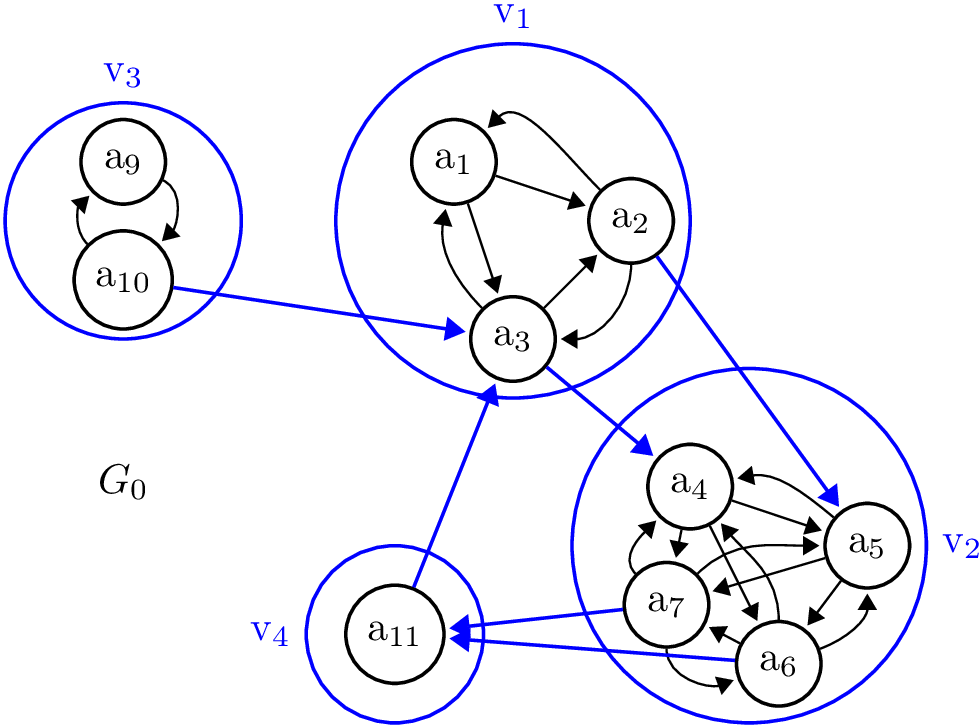
\includegraphics[scale=0.315]{immagini/graph0.png}
    };
    \node[canvas is zy plane at x=5,draw,fill=white] (g1) at (0,0) {
        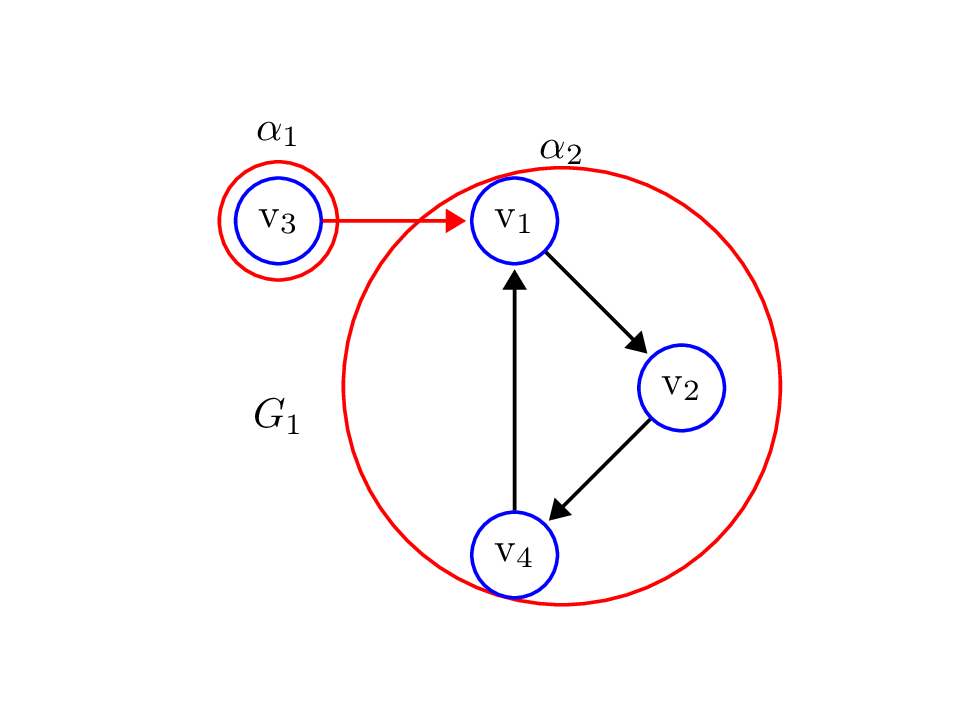
\includegraphics[scale=0.315]{immagini/graph1.png}
    };
    \node[canvas is zy plane at x=10,draw,fill=white] (g2) at (0,0) {
        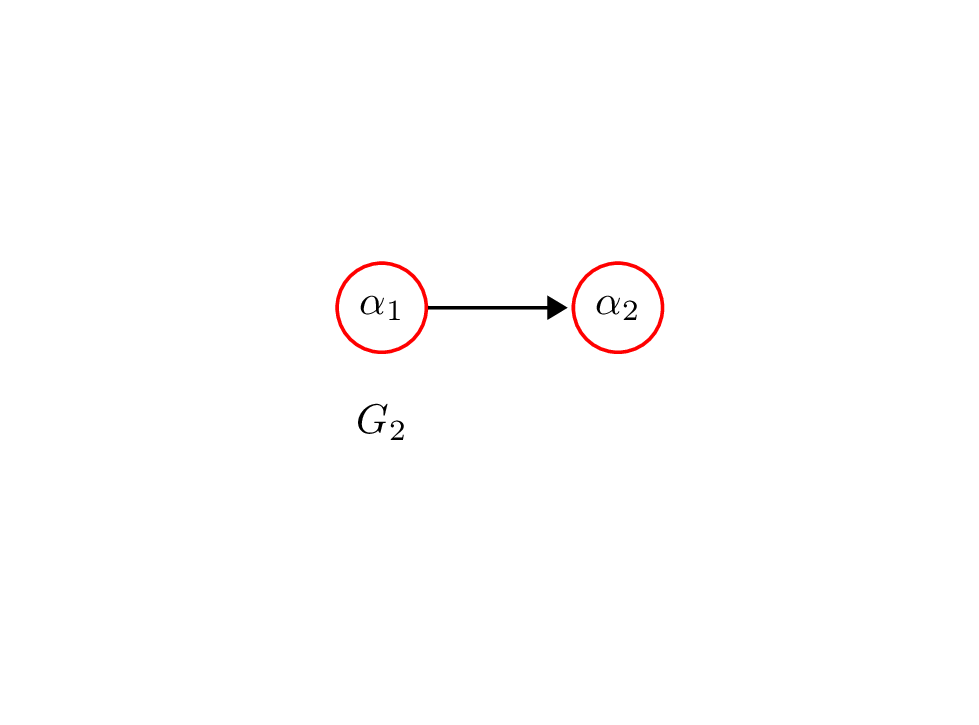
\includegraphics[scale=0.315]{immagini/graph2.png}
    };

    \node (G0) [below of=g0, node distance=5.2cm] {\huge $G_0$};
    \node (G1) [below of=g1, node distance=5.2cm] {\huge $G_1$};
    \node (G2) [below of=g2, node distance=5.2cm] {\huge $G_2$};

    \node (G0d) [below of=G0, node distance=1cm] {};
    \node (G1d) [below of=G1, node distance=1cm] {};
    \node (G2d) [below of=G2, node distance=1cm] {};

    \draw[->, line width=2pt, redUnicam] (G0d) -- (G1d) node[midway, below, red] {\huge $f_{C_1}$};
    \draw[->, line width=2pt, redUnicam] (G1d) -- (G2d) node[midway, below, red] {\huge $f_{C_2}$};
\end{tikzpicture}
        }
    \end{figure}
\end{minipage}
\end{frame}
}
%%%%%%%%%%%%%%%%%%%%%%%%%%%%%%%%%%%%%%%%%%%%%%%%%%%%%%
%%%%%%%%%%%%%%%%%%%%%%%%%%%%%%%%%%%%%%%%%%%%%%%%%%%%%%
\begin{frame}{Outline}
\tableofcontents
\end{frame}

%%%%%%%%%%%%%%%%%%%%%%%%%%%%%%%%%%%%%%%%%%%%%%%%%%%%%%
%%%%%%%%%%%%%%%%%%%%%%%%%%%%%%%%%%%%%%%%%%%%%%%%%%%%%%
\subsection{Complex Networks, Topological Data Analysis and Biology}
\begin{frame}{Complex Networks}
Complex networks are one of the most used tool for studying complex systems, weighted networks are becoming a more and more important tool to detect either the presence and the intensity of relations among groups of nodes in a network.

\centering{
%\includegraphics[width=0.50\textwidth]{immagini/complex}
}

\end{frame}
%%%%%%%%%%%%%%%%%%%%%%%%%%%%%%%%%%%%%%%%%%%%%%%%%%%%%%
%%%%%%%%%%%%%%%%%%%%%%%%%%%%%%%%%%%%%%%%%%%%%%%%%%%%%%


\section*{Acknowledgements}
\begin{frame}{Acknowledgements}
\begin{center}

\includegraphics[width=6.5cm]{./immagini/thanks}
\end{center}
\end{frame}

%%%%%%%%%%%%%%%%%%%%%%%%%%%%%%%%%%%%%%%%%%%%%%%%%%%%%%
%%%%%%%%%%%%%%%%%%%%%%%%%%%%%%%%%%%%%%%%%%%%%%%%%%%%%%

\end{document}
